\section{Overview}\label{s:overview}

\subsection{Detecting a hypervisor}\label{HV_detection}

While hypervisors by design are not easily detectable, there still exist many ways to detect the presence of them from the user-mode level. 
This paper could not cover all of the possible detection ways, but it does touch on the most commonly used methods.

%% Might look better to add a subsection for each of these parai sections(CPUID and RDTSC combined as x86 ASM instructions)
\parai{CPUID}
One of the most commonly used detection methods involve querying the CPUID instruction, defined in x86 architecture. 
This instruction returns information about the CPU and has multiple fields in the return data from which hypervisor identifiable information can be obtained. 
A more exhausting explanation of this instruction can be found in Intel\textsuperscript{\tiny\textregistered} 64 and IA-32 Architectures Software Developer's Manual~\cite[Volume~2A]{Intel-SDM2025}. Under a hypervisor, 
this instruction will always cause an unconditional VM-exit, and the hypervisor must have a handler present to correctly handle the instruction, 
which in most cases can be a passthrough to the logical CPU. Calling this instruction and reading specific bits of the return data is the easiest 
and most common way a process can detect the hypervisor, but this relies on the hypervisor itself writing this identifiable data before returning from the VMX root mode. 
A transparent hypervisor can be set up to pass through the instruction to the logical CPU for every query and the guest system could never detect this hypervisor from only the CPUID instruction.

\parai{RDTSC}
Another x86 instruction that causes an unconditional VM-exit in a virtualized environment is the RDTSC instruction. This instruction reads and returns the value of the time stamp counter, 
a register that counts the CPU cycles since it's reset. Its use in hypervisor detection is also common as it allows the detection of timing anomalies introduced by the aforementioned VM-exits 
and the transitions between non-root and root modes~\cite{hyperdbg-transparency}. This instruction called twice, before and after another instruction that causes a VM-exit, like CPUID, as seen here.
\begin{minted}[linenos,frame=single]{nasm}
    RDTSC
    CPUID
    RDTSC
\end{minted}

Subtracting values returned by the RDTSC instructions would show detectable overhead as the mode transitions, as well as the hypervisor itself, will execute more instructions and spend more CPU cycles than executing the same code in a bare metal system. 
As seen in Figure~\ref{fig:rdtsc_overhead}, the CPU cycle count it takes to execute the CPUID instruction is a lot larger when run in a VMWare virtualized environment than on bare metal. 
\begin{figure}[tbh]
    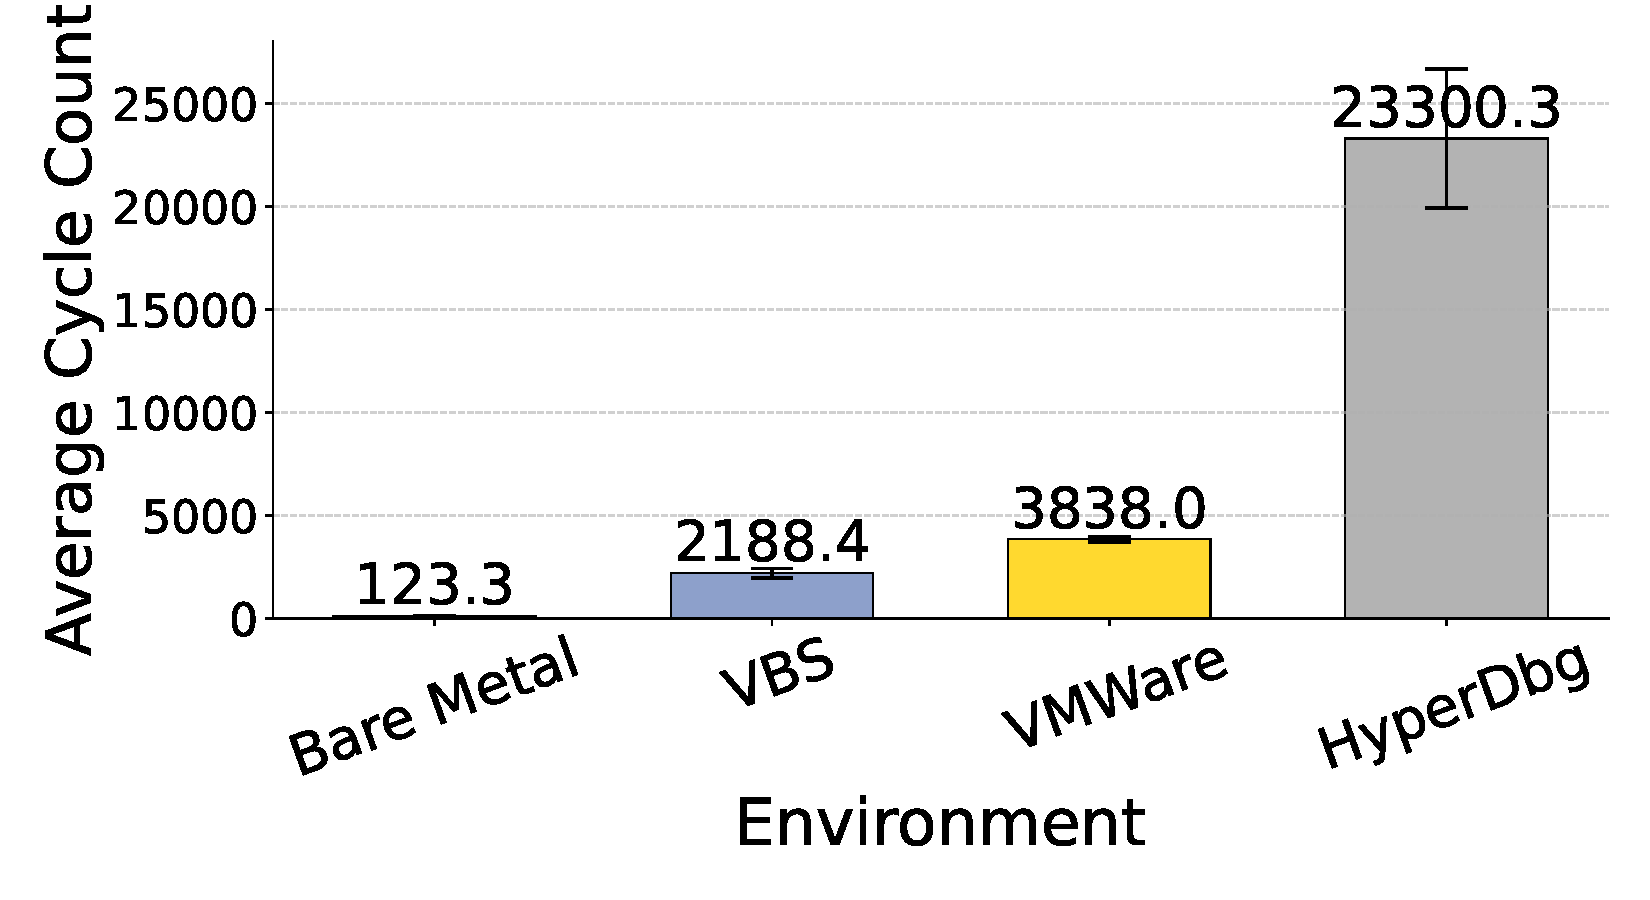
\includegraphics[width=\onecolgrid]{RDTSC_execution} %RDTSC_execution
    \figcap{Average cycle count of executing CPUID instruction in 4 different environments. VBS was tested on the same bare metal system and HyperDbg was run on top of a VMware system}\label{fig:rdtsc_overhead}
\end{figure}

It's also visible that HyperDbg's implementation of the CPUID instruction handler or the general VM-exit handler is a lot less efficient than VMWare's implementation, as the cycle count overhead is over 5 times larger. 
This detection method is reliable, as the overhead measurements are done in cycle count not time offset, and hard to defeat from the hypervisor as many genuine processes rely on the RDTSC 
instruction and the detection is done as a pattern not a singular query, making detecting the attempt of hypervisor detection unreliable and hard to implement~\cite{hypervisor-detection-timing-attacks}. 
The viability of this detection method, however, is no longer that high. In recent Windows operating system releases Microsoft has introduced Virtualization Based Security(VBS) feature~\cite{windows-vbs} 
that runs the operating system on top of a light hypervisor. This feature is enabled by default on modern Windows systems and introduces almost the same cycle count overhead, Figure~\ref{fig:rdtsc_overhead}. 
Malware that wants to target as many systems as it can or bypass this security feature, would have to sacrifice using the aforementioned detection method as it would blacklist and not deploy on not just the virtualized systems used for its analysis, 
but most bare metal systems as well. It should be noted that the overhead is smaller than the other hypervisors tested, but the difference is a lot smaller and differentiating them would be less reliable from the detection point of view. 

\parai{System calls}
When focusing on a specific guest operating system, detecting hypervisors can be done by using system calls provided by the OS. 
On Windows there are numerous ways how system calls could be used to assist in detecting them. This paper focused on the Windows system calls seen in Table~\ref{tab:syscalls}. 

The specific system call numbers were obtained from J00ru's Windows x64 syscall table~\cite{j00ruSyscalls} and they are based of Windows 11 version 24H2. All of these system calls can be invoked from a user-mode process and all of them can reveal the presence of a hypervisor in some way. 
Many of the calls focus on file and registry key access as commercial hypervisor vendors write identifiable data to the guest system. 
Mitigations to these attempts of detection are many, but the design developed as part of this paper focuses on intercepting the system calls at the OS kernel level 
and modifying the data the calling process receives if it contains hypervisor identifying data.

While these mitigations themselves try to stay hidden from the caller processes and the hypervisor might be transparent from the detection attempts, intercepting these calls comes with some design flaws that allow user processes to detect that
some intervention was performed, this will be mentioned in more detail in section~\ref{syscall_interception}.
For these mitigations, some system calls only require changing the return value, while others need intercepting pointers to user allocated buffers from the system call arguments and modifying the data inside these memory addresses.
The main issue with the use of system calls in hypervisor detection is that they are bound to a single operating system, and in the case of Windows possibly to a single version, as Microsoft tends to change the system call numbers over versions.
This version limitation, however, can be bypassed by using Windows API function calls for the wrapper functions of the system calls, but this approach is a lot easier to mitigate and can even be done in user-space, without a need for hypervisor intervention.

\begin{table}[tb]
    \centering
    \tabcap{Some Windows systemcalls with a possible use in hypervisor detection}\label{tab:syscalls}
    \taburulecolor{black!45}
    \begin{tabu}{l|c|c|c|c}
        \toprule
        \multirow{2}{*}{\thead{Name}} &
            \thead{System call} &
            \thead{Implemented} \\
        &
            \thead{number in 24H2} &
            \thead{in HyperDbg}\\
        \midrule
        NtQuerySystemInformation
            & 0x0036 & \checkmark \\
        NtSystemDebugControl
            & 0x01D0 & \checkmark\\
        NtQueryAttributesFile
            & 0x003D & \checkmark \\
        NtQueryObject
            & 0x0010 &\\
        NtOpenDirectoryObject
            & 0x0058 &\\
        NtQueryDirectoryObject
            & 0x014E & \checkmark\\
        NtQueryInformationProcess
            & 0x0019 & \checkmark \\
        NtQueryInformationThread
            & 0x0025 &\\
        NtOpenFile
            & 0x0033 & \checkmark\\
        NtOpenKey
            & 0x0012 & \checkmark \\
        NtQueryValueKey
            & 0x0017 & \checkmark \\
        NtEnumerateKey
            & 0x0032 & \checkmark \\
        NtUserFindWindowEx
        & 0x1067 &\\
        NtUserBuildHwndList
        & 0x101A &\\
        \bottomrule
    \end{tabu}

\end{table}

\parai{Model specific registers.}
Model specific registers(MSR) are special registers defined on the CPU that can be accessed only via special RDMSR and WRMSR instructions~\cite[Volume~4]{Intel-SDM2025}.
These MSR's hold different and more detailed data than the CPUID instruction, as well as specific control register fields. 
Importantly for hypervisor detection, the behavior of accessing specific MSR addresses or ranges is different when the system is virtualized 
as both the read and write instructions cause unconditional VM-exits and are handled by the hypervisor. Due to these instructions also being limited to privilege level 0, 
MSR access patterns are not as common as detection vectors, but if they are used, a positive test result guarantees a definitive detection of a hypervisor.

\parai{Other detection methods.}
This paper can only focus on a small number of hypervisor detection methods and their mitigations. There are uncountable ways to detect the presence of a virtual environment and as many ways to mitigate this.
Some other detection vectors might include checking I/O and other hardware device ID's and properties, reading the names of the system or the user account, checking system firmware data or executing hypervisor specific detection tests.
Mitigating all possible detection methods is near impossible, but at the same time, implementing and executing all these virtualization detection methods is inefficient in both time and space and can cause higher rates of false positives.


\subsection{Design approach}\label{design_approach}
Due to the complexity of the mitigations for some of these detection methods and the scope of this paper, only 3 general approaches to detection were handled, CPUID queries, MSR access patterns and Windows system calls. 
The hypervisor detection mitigation features were implemented into HyperDbg's transparency mode. 

By default, when HyperDbg is deployed, this feature and thus the ability to hide any hypervisors from detection, is disabled. To deploy the transparent mitigations, 
once HyperDbg is connected in kernel debug mode, “!hide” command needs to be entered. This enables all hypervisor detection mitigations that were implemented as part of this paper and, 
as it will be shown in the Evaluation section, improves the stealthiness of the hypervisors present. An overview of deploying the transparent mitigations with HyperDbg can be seen in Figure~\ref{fig:hyperdbg_overview}.

\begin{figure*}[t]
    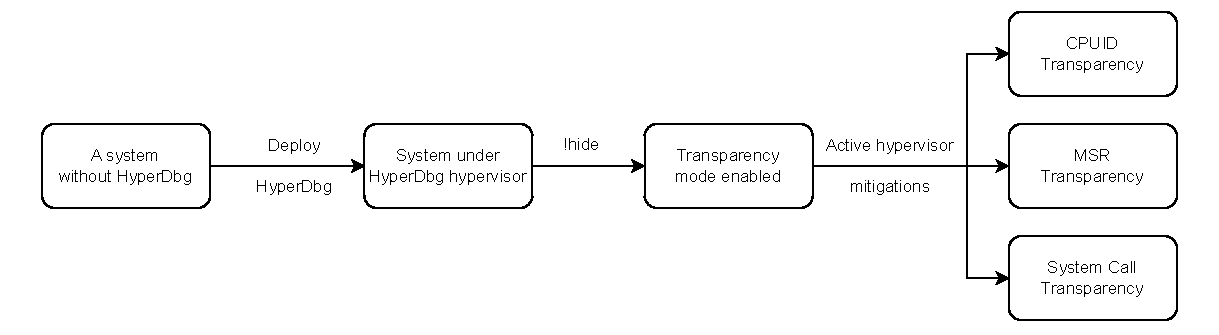
\includegraphics[width=\textwidth]{HyperDbg_diagram} %RDTSC_execution
    \figcap{Diagram of deploying the hypervisor transparency features implemented in HyperDbg}\label{fig:hyperdbg_overview}
\end{figure*}


%%% Local Variables:
%%% mode: latex
%%% TeX-master: "../thesis"
%%% End:
